%% Overview figure for the Computational Urban Science manuscript (Figure 1).
%% Standalone TikZ -> overview_figure.pdf, rasterised to wide_overview.png for
%% the manuscript build and converted to EPS for the journal.
%%
%% Top to bottom, three columns: what the map gives on the left, what the
%% timetable gives on the right, and what both share down the middle -- the
%% boundary, the travel-time constants, the pedestrian layer. The shape follows
%% the study, which is a paired comparison from end to end.
%%
%% On size. The figure is set to the column width, so what decides how much of
%% the page it eats is not its own dimensions but its aspect ratio: printed
%% height = column width x H/W. Scaling the drawing down changes nothing.
%% Height therefore comes out of rows and lines, never out of width:
%%
%%   * the boundary shares a row with the two sources instead of owning one,
%%     which is also what puts all three shared stages in the middle column;
%%   * every box is a heading and at most one line under it;
%%   * the closing sentence moved to the caption, where it costs no height.
%%
%% Style follows workflow_figure.tex: same muted print- and colourblind-safe
%% palette, same rounded stages, same Stealth arrows.
\documentclass[border=5pt]{standalone}
\usepackage[T1]{fontenc}
%% Nimbus Sans и Nimbus Mono -- контурные шрифты. Без второго 	exttt брал
%% cmtt, и dvips вкладывал его в EPS растровым Type 3, который в препрессе
%% печатается ступеньками.
\usepackage{helvet}
\usepackage{courier}
\renewcommand{\familydefault}{\sfdefault}
\usepackage{tikz}
\usetikzlibrary{arrows.meta, positioning, backgrounds, fit, calc}

% ---- palette shared with the library figure ----
\definecolor{dataBd}{HTML}{475569}\definecolor{dataFl}{HTML}{EEF2F7}
\definecolor{cutBd}{HTML}{B45309}\definecolor{cutFl}{HTML}{FBF0E3}
\definecolor{netBd}{HTML}{0F766E}\definecolor{netFl}{HTML}{DFF1EE}
\definecolor{fitBd}{HTML}{9A3412}\definecolor{fitFl}{HTML}{FDEDE3}
\definecolor{walkBd}{HTML}{6B7280}\definecolor{walkFl}{HTML}{F3F4F6}
\definecolor{outBd}{HTML}{2563A8}\definecolor{outFl}{HTML}{E7F0FA}

%% Кегли заданы числом, а не \footnotesize: рисунок печатается уменьшенным до
%% ширины полосы -- 17.1 см в 13.1, -- и журнал меряет буквы в этом, готовом
%% размере, где им положено 8--12 pt. 11 pt на холсте дают 8.4.
\newcommand{\hd}{\fontsize{11.5}{13}\selectfont\bfseries}
\newcommand{\sub}[1]{\\[1.5pt]{\fontsize{10.5}{12}\selectfont #1}}

\begin{document}
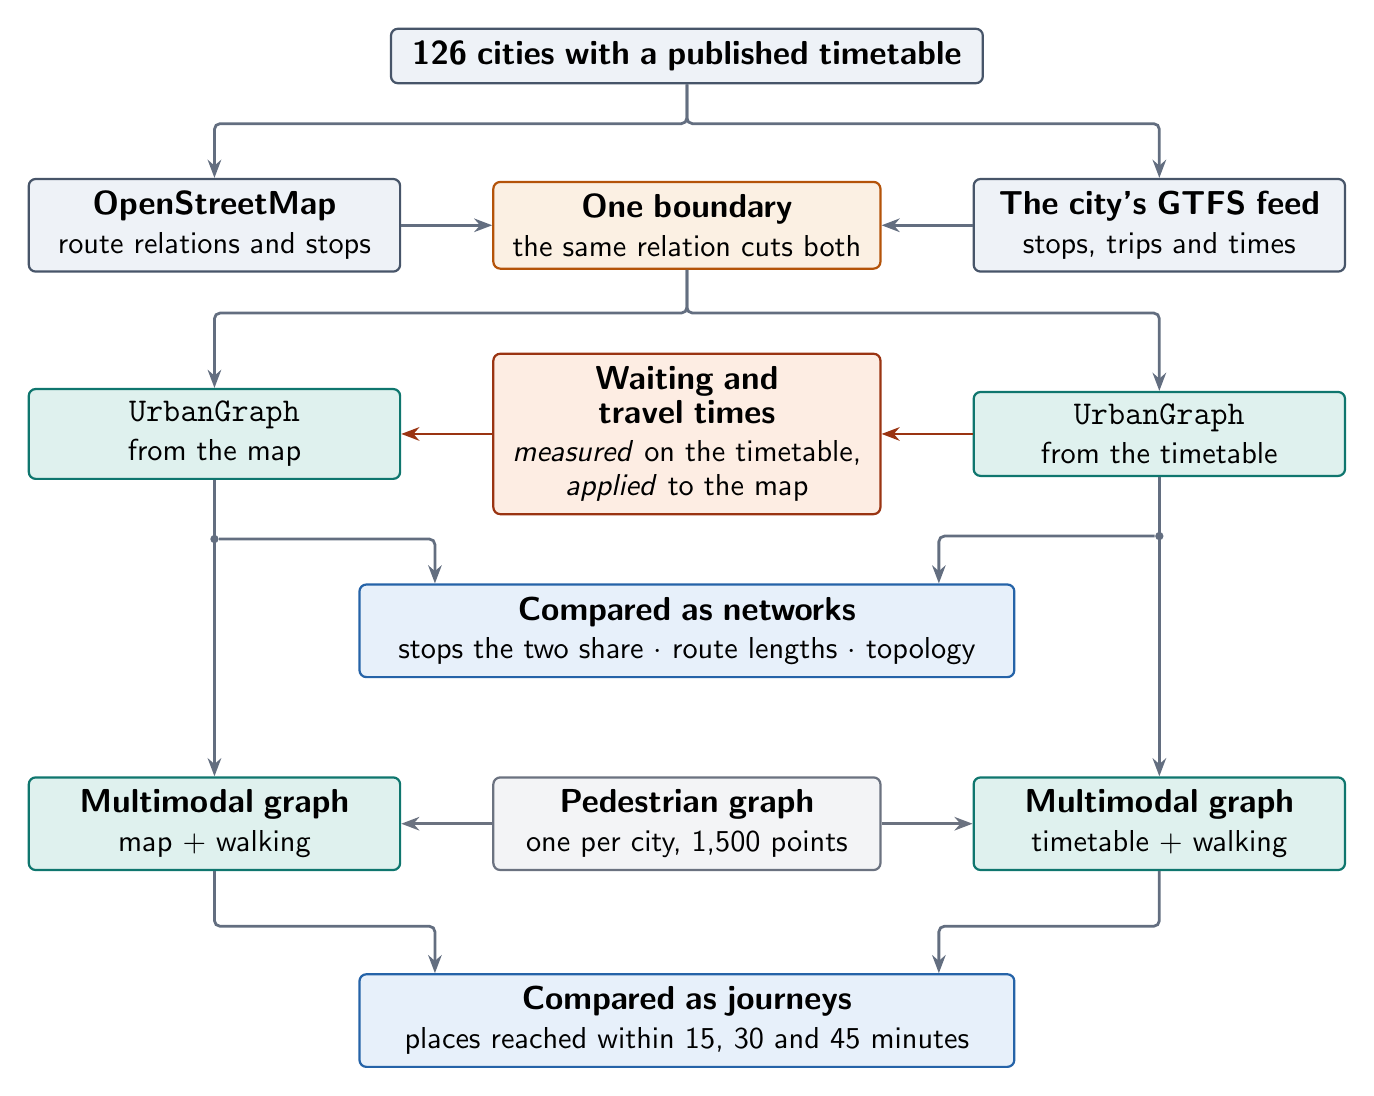
\begin{tikzpicture}[
  font=\fontsize{11}{12.5}\selectfont,
  >={Stealth[length=2.3mm]},
  box/.style={rounded corners=2.5pt, draw, line width=0.8pt, align=center,
              inner sep=4.5pt},
  flow/.style={->, line width=1.0pt, draw=dataBd!85, rounded corners=2pt},
  side/.style={->, line width=1.0pt, draw=fitBd, rounded corners=2pt},
  walkflow/.style={->, line width=1.0pt, draw=walkBd, rounded corners=2pt},
  tap/.style={circle, fill=dataBd!85, inner sep=0pt, minimum size=3pt},
]

% ---------------------------- the cohort ----------------------------------
\node[box, draw=dataBd, fill=dataFl, text width=7.2cm] (cities) at (0,0)
  {{\hd 126 cities with a published timetable}};

% ------------------- the two sources, cut by one boundary -----------------
\node[box, draw=dataBd, fill=dataFl, text width=4.4cm] (osm) at (-6.0cm,-2.15cm)
  {{\hd OpenStreetMap}\sub{route relations and stops}};

\node[box, draw=dataBd, fill=dataFl, text width=4.4cm] (gtfs) at (6.0cm,-2.15cm)
  {{\hd The city's GTFS feed}\sub{stops, trips and times}};

\node[box, draw=cutBd, fill=cutFl, text width=4.6cm] (clip) at (0,-2.15cm)
  {{\hd One boundary}\sub{the same relation cuts both}};

% ---------------------------- the two graphs ------------------------------
\node[box, draw=netBd, fill=netFl, text width=4.4cm] (ugosm) at (-6.0cm,-4.80cm)
  {{\hd\texttt{UrbanGraph}}\sub{from the map}};

\node[box, draw=netBd, fill=netFl, text width=4.4cm] (ugfeed) at (6.0cm,-4.80cm)
  {{\hd\texttt{UrbanGraph}}\sub{from the timetable}};

\node[box, draw=fitBd, fill=fitFl, text width=4.6cm] (coef) at (0,-4.80cm)
  {{\hd Waiting and travel times}
   \sub{\textit{measured} on the timetable,\\ \textit{applied} to the map}};

% ---------------------------- first comparison ----------------------------
\node[box, draw=outBd, fill=outFl, text width=8.0cm] (topo) at (0,-7.30cm)
  {{\hd Compared as networks}
   \sub{stops the two share $\cdot$ route lengths $\cdot$ topology}};

% ------------------- multimodal graphs over one pedestrian layer ----------
\node[box, draw=netBd, fill=netFl, text width=4.4cm] (mmosm) at (-6.0cm,-9.75cm)
  {{\hd Multimodal graph}\sub{map $+$ walking}};

\node[box, draw=netBd, fill=netFl, text width=4.4cm] (mmfeed) at (6.0cm,-9.75cm)
  {{\hd Multimodal graph}\sub{timetable $+$ walking}};

\node[box, draw=walkBd, fill=walkFl, text width=4.6cm] (walk) at (0,-9.75cm)
  {{\hd Pedestrian graph}\sub{one per city, 1,500 points}};

% ---------------------------- second comparison ---------------------------
\node[box, draw=outBd, fill=outFl, text width=8.0cm] (acc) at (0,-12.25cm)
  {{\hd Compared as journeys}
   \sub{places reached within 15, 30 and 45 minutes}};

% ---------------------------- flow ----------------------------------------
% The cohort forks over the boundary box, which sits in the same row.
\draw[flow] (cities.south) -- ++(0,-0.5cm) -| (osm.north);
\draw[flow] (cities.south) -- ++(0,-0.5cm) -| (gtfs.north);

\draw[flow] (osm.east)   -- (clip.west);
\draw[flow] (gtfs.west)  -- (clip.east);

\draw[flow] (clip.south) -- ++(0,-0.55cm) -| (ugosm.north);
\draw[flow] (clip.south) -- ++(0,-0.55cm) -| (ugfeed.north);

% The timetable pays for the constants the map has no way to state; the two
% directions are named inside the box, where a 1.6 cm arrow has no room for a
% label of its own.
\draw[side] (ugfeed.west) -- (coef.east);
\draw[side] (coef.west)   -- (ugosm.east);

% Each graph runs straight down its own track; the first comparison taps that
% line instead of taking a second arrow off the box.
\draw[flow] (ugosm.south)  -- (mmosm.north);
\draw[flow] (ugfeed.south) -- (mmfeed.north);

\node[tap] (tapL) at ($(ugosm.south)+(0,-0.75cm)$) {};
\node[tap] (tapR) at ($(ugfeed.south)+(0,-0.75cm)$) {};
\draw[flow] (tapL) -| ([xshift=-3.2cm]topo.north);
\draw[flow] (tapR) -| ([xshift=3.2cm]topo.north);

% the pedestrian layer joins both, the way the constants did above
\draw[walkflow] (walk.west) -- (mmosm.east);
\draw[walkflow] (walk.east) -- (mmfeed.west);

\draw[flow] (mmosm.south)  -- ++(0,-0.7cm) -| ([xshift=-3.2cm]acc.north);
\draw[flow] (mmfeed.south) -- ++(0,-0.7cm) -| ([xshift=3.2cm]acc.north);

\end{tikzpicture}
\end{document}
